\documentclass[12pt]{article}  % [12pt] option for the benefit of aging markers

% amssymb package contains more mathematical symbols
\usepackage{amssymb,amsthm}
\usepackage{hyperref}

% graphicx package enables you to paste in graphics
\usepackage{graphicx}
\usepackage{auto-pst-pdf}

% embed source inside latex
\usepackage[procnames]{listings}
\usepackage{color}

%%%%%%%%%%%%%%%%%%%%%%%%%%%%%%%%%
%
%    Page size commands.  Don't worry about these
%
\setlength{\textheight}{220mm}
\setlength{\topmargin}{-10mm}
\setlength{\textwidth}{150mm}
\setlength{\oddsidemargin}{0mm}

%%%%%%%%%%%%%%%%%%%%%%%%%%%%%%%%%%%%%%%%%%%%%%%%%%%%%%%%%%%%%%%
%
%    Definitions of environments for theorems etc.
%
\newtheorem{theorem}{Theorem}[section]          % Theorems numbered within sections - eg Theorem 2.1 in Section 2.
\newtheorem{corollary}[theorem]{Corollary}      % Corollaries etc. will be counted as Theorems for numbering
\newtheorem{lemma}[theorem]{Lemma}              % eg Lemma 3.1, ... Theorem 3.2, ... Corollary 3.3.
\newtheorem{proposition}[theorem]{Proposition}
\newtheorem{conjecture}[theorem]{Conjecture}

\theoremstyle{definition}
\newtheorem{definition}[theorem]{Definition}

\theoremstyle{remark}
\newtheorem{remark}[theorem]{Remark}
\newtheorem{example}[theorem]{Example} 

%%%%%%%%%%%%%%%%%%%%%%%%%%%%%%%%%%%%%%%%%%%%%%%
%
%        Preamble material specific to your essay
%
\title{Network Topology Discovery}
\author{Yan Jiaqi\\
A20321362\\
CS542 Project\\
Lectured by Prof. Edward Chlebus}

\begin{document}
\maketitle

% \newpage                     % optional page break
\begin{abstract}
In this project, we first propose the content of topology update message for correct topology discovery.
The \textit{portion of the network seen by a router} is used to quantify the efficiency of the network update process.
A small scale network built by 6 routers is simulated to demonstrate the process of populating topology information.
The simulation, as well as the distributed discovery algorithm, should terminate when every router's \textit{topology database} is stable.
Simulation results are shown for both router $R_1$ and router $R_6$.
\end{abstract}

\newpage                     % optional page break
\tableofcontents

\newpage                     % optional page break
\section{Problem Statement}\label{s:intro}
%
% The \label command is optional, but useful.  To cross-refer to a section/theorem/equation etc.
% labelled by \label{key}, use \ref{key}.  For example: Equation (\ref{eq:key}) follows from Theorem \ref{th:key}.

In this project, we explore the problem of letting distributed routers know the entire network topology.
As the `God' of the network, we network operator have the global view of the network.
The routers, however, only knows its direct neighbors.
Since we are considering unidirectional links, \textbf{neighbors} of a particular router $r$ can fall into one of two cases: the one that can be reached from $r$ and the one that can reach $r$.

The problem can be stated more formally as follows. The network topology as the adjacent matrix $AM$ is given to us.
An example which we will simulate is shown below:
\begin{center}
\begin{tabular}{|r|r|r|r|r|r|r|}        % 7 columns, each right-justified
\hline                                  % horizontal line between rows
 & $R_1$ & $R_2$ & $R_3$ & $R_4$ & $R_5$ & $R_6$ \\ % header row
\hline
$R_1$ &   & 3 &   &   &    & \\
\hline
$R_2$ & 4 &   & 6 &   &    & \\
\hline
$R_3$ &   &   &   & 7 &    & \\
\hline
$R_4$ &   &   &   &   & 11 & \\
\hline
$R_5$ &   &   &   &   &    & 9 \\
\hline
$R_6$ &   & 8 & 5 &   &    & \\
\hline
\end{tabular}
\end{center}
The cost from source router $s$ to destination $d$ is given as $AM[s][d]$.
Empty cell means the cost is $\infty$, meaning no link exist between router $s$ and $d$.
Every router $r$ maintain its \textbf{topology database}.
Initially, this database in a given router $r$ contains only row $r$ and column $r$ in matrix $AM$ because
\begin{itemize}
        \item $r$ is aware the routers it can directly go to, corresponding to row $AM[r][0..N-1]$, all the outgoing links.
        \item $r$ knows the routers that can directly go to itself, corresponding to column $AM[0..N-1][r]$, all the incoming links.
\end{itemize}

The problem is: how to let each router has the entire topology matrix or database?
The motivation is that if a router has the complete topology matrix, it can further run Dijkstra's algorithm to obtain a shortest path tree, whose root is the router $r$ itself.
Next hop for any network or any other router can then be obtained from this shortest path tree.
In other words, it can automatically and dynamically create/update its routing table\footnote{Just out of my interest, I implemented the procedure of routing table creation based on Dijkstra's shortest path algorithm.
Not described in this report but can be found in the source code for router}.

\section{Discovery Process}

\subsection{Message Format}
The solution to topology discovery itself is simple.
Every router advertises its current known links (column and row in its incomplete database) to its downstream neighbors.
Each advertising message consists of 2 parts.

The first field $k_m$ is called the key of the message.
It is a unique ID for a router in the network, which, playing as a \textit{key}, indicates the row index and column index in the imaginary topology matrix.

Then goes the links encapsulated inside the message.
It is a 2-element tuple containing associated links of the router identified by the key $k_m$.
In terms of topology matrix, this tuple contains the row and the column corresponding to this keyed router.
Both elements in this tuple are key-value map structure: the keys are still a router ID and its values are the cost of links.
However, the interpretation of the cost is different for the 1st and 2nd element in this tuple.
The 1st elements specifies the cost of outing links while the 2nd element specifies the incoming links.
For example, the cost value associated with a key $k_1$ in the first element represents the cost from router $k_m$ to router $k_1$;
for the cost value associated with $k_2$ in the second element, it represents the cost from router $k_2$ to router $k_m$.

An advertisement in one iteration from any router may contains a sequence of such messages if the source router has more than 1 record in its database.
Once a router receives advertisements from other routers, it checks if there is anything new to its own database.
If yes, it inserts a record, the (outgoing link cost, incoming link cost) tuple to its database with the key of the message as table index.

\subsection{Measuring the Discovery Process}
An obvious metric is the percentage of the network topology matrix a router currently has.
For the example mentioned above, at the initial stage, every router only knows 1 row and 1 column of the matrix.
So everyone starts from percentage $1/N$ where $N$ is total number of routers in the network.
At iteration $n=1$, $R_2$ received messages from router $R_1$ and $R_6$; then it has 3 rows and 3 colums, which means 50\% of the network is known to $R_2$.

\section{Simulation and Termination}
We can simulate the distributed discovery process.
Simulation's basic flow is shown in Listing \ref{lst:while-loop}.
Notice that this simulation assume that all routers are \textbf{synchronized} after each iteration.

\subsection{Termination}
The discovery step is repeated until all of the routers' topology database is stable.
That is, we jump out of the while-loop when the boolean variable $updated$ is never set to $True$ when any router $r$ invokes \texttt{update\_topo()}.
The reason is simple: if every router's topology database is identical, no new information will be transferred between each other.
At this moment, all routers must have the same and correct network view, except for that something happened after the population ends.

In fact, if assuming that no change happens during the topology discovery/update process, it will always terminate in $L$ iterations, where $L$ is the length of the longest path in the network graph.
Therefore, the worst case time complexity of this distributed algorithm is bounded by $O(N)$, where $N$ is the number of routers in the graph.
In the case that network is changed, just restart the discovery process at each router and wait for them to converge again.
This topology update process can also be done incrementally.

\subsection{Code Structure}
Inside the while-loop of simulation, we have a scatter-gather pattern.
In the scatter phase, router $r$ will receive messages from its each neighbors $n$ who can reach $r$ directly.
In the gathering phase, each router update its topology databased by handling the received messages, which is stored inside its buffer at the scatter phase.
The processing is very simple: if router $r$ have seen a message with unknown key, it inserts the links inside this message to its database with this unseen key.

% Python code embedding configuration
\definecolor{keywords}{RGB}{255,0,90}
\definecolor{comments}{RGB}{0,0,113}
\definecolor{red}{RGB}{160,0,0}
\definecolor{green}{RGB}{0,150,0}
\lstset{language=Python,
        basicstyle=\ttfamily\small,
        keywordstyle=\color{keywords},
        commentstyle=\color{comments},
        stringstyle=\color{red},
        showstringspaces=false,
        identifierstyle=\color{green},
        procnamekeys={def,class,True},
        frame=single,
        numbers=left,
        numbersep=5pt,
        numberstyle=\tiny\color{blue},
        rulecolor=\color{black},
        caption={Simulation Discovery Process},
        label=lst:while-loop,
        language=Python,
}
\begin{lstlisting}
while updated:
    for r in routers:
        for n in r.neighbors:
            router_n = get_router_by_name(n, routers)
            # send items in topology database one by one
            for n_name, n_row_col in router_n.topo.items():
                n_msg = (n_name, n_row_col)
                r.recv_msg(n_msg)
    updated = False
    for r in routers:
        if r.update_topo_database():
            # something new is added to a router
            updated = True
\end{lstlisting}

\section{Experiment Results}
In this section, the discovery progresses for router $R_1$ and $R_6$ are shown.

In the log that shows each iteration result, we use ``()" to group elements in tuple structure;
we use ``\{\}" to group a sequence of key-value items and ``:" to separate key with value.
For example, $(e_1, e_2, e_3)$ is a tuple with 3 elements;
$\{k_1:v_1, k_2:v_2\}$ is a dictionary contains 2 key-value items;
$(\{k_{11}:v_{11}, k_{12}:v_{12}\},\{k_{21}:k_{22}\})$ is a tuple of two dictionaries.
This syntax is entirely adopted from Python's programming syntax.

The topology database of a router at a particular iteration is printed out as a list of tuples, surrounded by ``[]" symbols.
Each tuple represent a record of the database, first element as index and second element as content.
The content is a two-element tuple depict link information.

\subsection{Results for $R_1$}
At each iteration, the snapshot of $R_1$'s topology database is shown in Listing \ref{lst:r1}.
Each entry in the database is indexed by router name or id.
Inside the entry stores the links, both outgoing and incoming type, of the index router.
For example, at the 3rd iteration, $R_1$ found out 3 other routers exist in the network.
One of them is called $R6$, who can reach $R_2$ and $R_3$ with cost 8 and 5 respectively;
also this $R_6$ can be reached from another router $R_5$ with cost 9.
At 5th iteration and 6th iteration, $R_1$ has the same topology database.
In fact all routers at the 6th iteration have the same topology database and meet the termination requirement.
This stable database is also the complete representation of the network.

\lstset{basicstyle=\ttfamily\small,
        keywordstyle=\color{keywords},
        commentstyle=\color{comments},
        stringstyle=\color{red},
        showstringspaces=false,
        identifierstyle=\color{green},
        procnamekeys={def,class},
        frame=single,
        numbers=left,
        numbersep=5pt,
        numberstyle=\tiny\color{blue},
        rulecolor=\color{black},
        caption={$R_1$'s Topology at Each Iteration},
        label=lst:r1,
        language=Python}
\begin{lstlisting}
0  [  ('r1', ({'r2': 3}, {'r2': 4}))  ]
1  [  ('r1', ({'r2': 3}, {'r2': 4})),
      ('r2', ({'r1': 4, 'r3': 6}, {'r6': 8, 'r1': 3}))  ]
2  [  ('r1', ({'r2': 3}, {'r2': 4})),
      ('r2', ({'r1': 4, 'r3': 6}, {'r6': 8, 'r1': 3})),
      ('r6', ({'r2': 8, 'r3': 5}, {'r5': 9}))  ]
3  [  ('r1', ({'r2': 3}, {'r2': 4})),
      ('r2', ({'r1': 4, 'r3': 6}, {'r6': 8, 'r1': 3})),
      ('r5', ({'r6': 9}, {'r4': 11})),
      ('r6', ({'r2': 8, 'r3': 5}, {'r5': 9}))  ]
4  [  ('r1', ({'r2': 3}, {'r2': 4})),
      ('r2', ({'r1': 4, 'r3': 6}, {'r6': 8, 'r1': 3})),
      ('r4', ({'r5': 11}, {'r3': 7})),
      ('r5', ({'r6': 9}, {'r4': 11})),
      ('r6', ({'r2': 8, 'r3': 5}, {'r5': 9}))  ]
5  [  ('r1', ({'r2': 3}, {'r2': 4})),
      ('r2', ({'r1': 4, 'r3': 6}, {'r6': 8, 'r1': 3})),
      ('r3', ({'r4': 7}, {'r6': 5, 'r2': 6})),
      ('r4', ({'r5': 11}, {'r3': 7})),
      ('r5', ({'r6': 9}, {'r4': 11})),
      ('r6', ({'r2': 8, 'r3': 5}, {'r5': 9}))  ]
6  [  ('r1', ({'r2': 3}, {'r2': 4})),
      ('r2', ({'r1': 4, 'r3': 6}, {'r6': 8, 'r1': 3})),
      ('r3', ({'r4': 7}, {'r6': 5, 'r2': 6})),
      ('r4', ({'r5': 11}, {'r3': 7})),
      ('r5', ({'r6': 9}, {'r4': 11})),
      ('r6', ({'r2': 8, 'r3': 5}, {'r5': 9}))  ]
\end{lstlisting}


\subsection{Results for $R_6$}
At each iteration, the snapshot of $R_6$'s topology database is shown in Listing \ref{lst:r6}.
For example, at the 3rd iteration, $R_1$ found out 3 other routers exist in the network.
One of them is called $R_3$, who can reach $R_4$ with cost 7;
also this $R_3$ can be reached from either router $R_6$ with cost 5 or router $R_2$ with cost 6.
At 5th iteration and 6th iteration, $R_6$ has the same topology database.
In fact all routers at the 6th iteration have the same topology database and meet the termination requirement.
So the number of iterations is 7 for our simulation.

\lstset{basicstyle=\ttfamily\small,
        keywordstyle=\color{keywords},
        commentstyle=\color{comments},
        stringstyle=\color{red},
        showstringspaces=false,
        identifierstyle=\color{green},
        procnamekeys={def,class},
        frame=single,
        numbers=left,
        numbersep=5pt,
        numberstyle=\tiny\color{blue},
        rulecolor=\color{black},
        caption={$R_6$'s Topology at Each Iteration},
        label=lst:r6,
        language=Python}
\begin{lstlisting}
0  [  ('r6', ({'r2': 8, 'r3': 5}, {'r5': 9}))  ]
1  [  ('r5', ({'r6': 9}, {'r4': 11})),
      ('r6', ({'r2': 8, 'r3': 5}, {'r5': 9}))  ]
2  [  ('r4', ({'r5': 11}, {'r3': 7})),
      ('r5', ({'r6': 9}, {'r4': 11})),
      ('r6', ({'r2': 8, 'r3': 5}, {'r5': 9}))  ]
3  [  ('r3', ({'r4': 7}, {'r6': 5, 'r2': 6})),
      ('r4', ({'r5': 11}, {'r3': 7})),
      ('r5', ({'r6': 9}, {'r4': 11})),
      ('r6', ({'r2': 8, 'r3': 5}, {'r5': 9}))  ]
4  [  ('r2', ({'r1': 4, 'r3': 6}, {'r6': 8, 'r1': 3})),
      ('r3', ({'r4': 7}, {'r6': 5, 'r2': 6})),
      ('r4', ({'r5': 11}, {'r3': 7})),
      ('r5', ({'r6': 9}, {'r4': 11})),
      ('r6', ({'r2': 8, 'r3': 5}, {'r5': 9}))  ]
5  [  ('r1', ({'r2': 3}, {'r2': 4})),
      ('r2', ({'r1': 4, 'r3': 6}, {'r6': 8, 'r1': 3})),
      ('r3', ({'r4': 7}, {'r6': 5, 'r2': 6})),
      ('r4', ({'r5': 11}, {'r3': 7})),
      ('r5', ({'r6': 9}, {'r4': 11})),
      ('r6', ({'r2': 8, 'r3': 5}, {'r5': 9}))  ]
6  [  ('r1', ({'r2': 3}, {'r2': 4})),
      ('r2', ({'r1': 4, 'r3': 6}, {'r6': 8, 'r1': 3})),
      ('r3', ({'r4': 7}, {'r6': 5, 'r2': 6})),
      ('r4', ({'r5': 11}, {'r3': 7})),
      ('r5', ({'r6': 9}, {'r4': 11})),
      ('r6', ({'r2': 8, 'r3': 5}, {'r5': 9}))  ]
\end{lstlisting}

\subsection{Discovery Percentage as a function of the iteration number}
As a function of iteration, the percentage of network discovered by both router $R_1$ and $R_6$ is shown in Figure \ref{fig:progress}.
The iteration number begins from 0 and ends at 6, an extra iteration to ensure that all routers in this network hold identical topology database.
As we can see the progress grows linearly at each iteration: at each step, router $R_1$ and $R_6$ found a new router and its links.

\begin{figure}[h]
\centering
        \includegraphics[scale=0.6]{progress.ps}
\caption{Discovery Percentage as Function of Iteration for $R_1$ and $R_6$}
\label{fig:progress}
\end{figure}

\appendix
\section{Source Code Printout}
The printout of all source code used in this project.
\lstinputlisting[language=Python, caption={Source Code for Router: \lstname}]{drrouter.py}
\lstinputlisting[language=Python, caption={Source Code for Simulation, \lstname}]{topology.py}


%%%%%%%%%%%%%%%%%%%%%%%%%%%%%%%%%%%%%%%%%
%
%     Bibliography
%
%     Use an easy-to-remember tag for each entry - eg \bibitem{How97} for an article/book by Howie in 1997
%     To cite this publication in your text, write \cite{How97}.  To include more details such as
%     page, Chapter, Theorem numbers, use the form \cite[Theorem 6.3, page 42]{How97}.
%
%\begin{thebibliography}{99}

% 
% The usual convention for mathematical bibliographies is to list alphabetically
% by first-named author (then second, third  etc. author then date)
% websites with no author names should go by the site name
%


% Typical layout for reference to a journal article
%
%\bibitem{Bovey}
%J. D. Bovey, M. M. Dodson,                         % author(s)
%The Hausdorff dimension of systems of linear forms % article name
%{\em Acta Arithmetica}                             % journal name - italics
%{\bf 45}                                           % volume number - bold
%(1986), 337--358.                                   % (year), page range

%% Typical layout for reference to a book
%%
%\bibitem{Cassels}
%J. W. S. Cassels,                                  % author(s)
%{\em An Introduction to Diophantine Approximation},% title - italics
%Cambridge University Press, Cambridge, 1965.       % Publisher, place, date.

%% Typical layout for reference to a website
%%
%\bibitem{GAP}
%The GAP Group, GAP -- Groups, Algorithms, and Programming,  % Site name
%Version 4.5.6; 2012. % other information
%(http://www.gap-system.org)  % URL


%% Typical layout for reference to an online article
%%
%\bibitem{Howie}
%J. Howie,                                            % author(s)
%{\em Generalised triangle groups of type $(3,5,2)$}, % article name - italics
%http://arxiv.org/abs/1102.2073                       % URL
%(2011).                                              % (year)
%\end{thebibliography}

\end{document}
